%&../settings/preamble.main

\ifsubfile
\usepackage{../settings/subfile}
\setcounter{chapter}{20}

\usepackage[newfloat, cachedir=_minted-cache, outputdir=../build]{minted}
\usepackage{../libraries/set-minted}

% \usepackage{debug}

% arara: pdflatex: { options: ["--output-directory=../build"], shell: yes, draft: yes, synctex: no }
% arara: pdflatex: { options: ["--output-directory=../build"], shell: yes, synctex: no }
\begin{document}
\fi


\chapter{Riassunto}

\section*{Risoluzione di problemi}

Dato un problema non esistono \enquote{ricette originali} per risolverlo in modo efficiente;
tuttavia è possibile evidenziare quattro fasi:
\begin{enumerate}
	\item \textbf{classificazione del problema}: è il primo passo verso la risoluzione;
	\item \textbf{caratterizzazione della soluzione}: bisogna caratterizzare matematicamente la soluzione, evitando di escludere soluzioni banali;
	\item \textbf{tecnica di progetto}: quando è possibile dividere il problema in più sottoproblemi di complessità minore allora la tecnica \enquote{divide et impera} potrebbe essere quella più appropriata (più avanti vedremo delle tecniche più interessanti quali: programmazione dinamica (Capitolo 13), algoritmi ingordi (Capitolo 14) e backtrack (Capitolo 16));
	\item \textbf{utilizzo di strutture dati}: bisogna scegliere la struttura dati più adatta alla risoluzione del nostro particolare problema (spesso sarà una tabella hash o un albero binario di ricerca, più avanti vedremo delle strutture dati specializzate per risolvere problemi specifici, a differenza di quelle che abbiamo visto fin'ora che sono generiche).
\end{enumerate}
Queste fasi non sono necessariamente sequenziali, l'ordine dipende da come stiamo affrontando il problema.

\subsection*{Classificazione dei problemi}

Ma come possiamo classificare un problema?
Le classi di problemi che affronteremo possono essere raggruppate in quattro macro-categorie:
\begin{itemize}
	\item \textbf{problemi decisionali}: consistono nel determinare se il dato in ingresso soddisfa o meno una certa proprietà ed hanno una risposta binaria (si/no, true/false); come ad esempio stabilire se un grafo risulta connesso o meno.
	Su questo genere di problemi spesso non esistono delle tecniche standard e bisogna creare algoritmi ad-hoc;
	\item \textbf{problemi di ricerca}: consistono nel trovare nello spazio di soluzioni possibili una soluzione ammissibile che rispetti certi vincoli, come ad esempio la ricerca della posizione di una sottostringa in una stringa.
	In questi problemi la tecnica \enquote{divide et impera} può rincorrere in nostro aiuto;
	\item \textbf{problemi di ottimizzazione}: ad ogni soluzione è associata una funzione di costo e vogliamo trovare quella di costo minimo, come ad esempio il cammino (pesato) più breve fra due nodi.
	Questa classe di problemi può essere risolta tramite la programmazione dinamica o algoritmi ingordi;
	\item \textbf{problemi di approssimazione}: a volte, trovare la soluzione ottima è computazionalmente impossibile e ci si accontenta di una soluzione approssimata, in questo caso il costo rimane basso ma non sappiamo se è ottimale; un esempio di questo genere di problemi è quello del commesso viaggiatore.
\end{itemize}

\subsection*{Caratterizzazione della soluzione}

\`{E} fondamentale definire bene il problema dal punto di vista matematico.
La formulazione del problema può suggerire una prima idea, seppur banale, alla risoluzione dello stesso.
Lo si può osservare nella formulazione del seguente problema: data una sequenza di \(n\) elementi, una permutazione ordinata è data dal minimo seguito da una permutazione ordinata dei restanti \(n-1\) elementi.
Questa formulazione produce l'algoritmo \selectionSort.
La definizione matematica può suggerire una possibile tecnica, ad esempio:
\begin{itemize}
	\item se troveremo una \emph{sottostruttura ottima} allora potremmo applicare la programmazione dinamica (Capitolo 13);
	\item se troveremo la \emph{proprietà greedy} allora potremmo applicare un algoritmo ingordo (Capitolo 14).
\end{itemize}

\section*{Tecniche di soluzione dei problemi}

Come vengono affrontati i problemi dalle varie tecniche?
\begin{itemize}
	\item nella \textbf{tecnica divide-et-impera} un problema viene suddiviso in sotto-problemi indipendenti, i quali vengono risolti ricorsivamente (avendo quindi un approccio dall'alto verso il basso, detto \foreign{top-down}); Abbiamo già visto diversi esempi dell'applicazione di questa tecnica, provate a pensare all'algoritmo \mergeSort: ordinare due sottovettori sono due problemi indipendenti (ordinare il sottovettore di sinistra non richiede conoscere il contenuto del vettore di destra e viceversa);
	\item nella \textbf{programmazione dinamica} la soluzione viene costruita (dal basso verso l'altro, \foreign{bottom-up}) a partire da un insieme di sotto-problemi potenzialmente ripetuti.
	\item la tecnica della \foreign{memoization} (annotazione) è la versione \foreign{top-down} della programmazione dinamica.
	\begin{figure}[H]
        \centering
        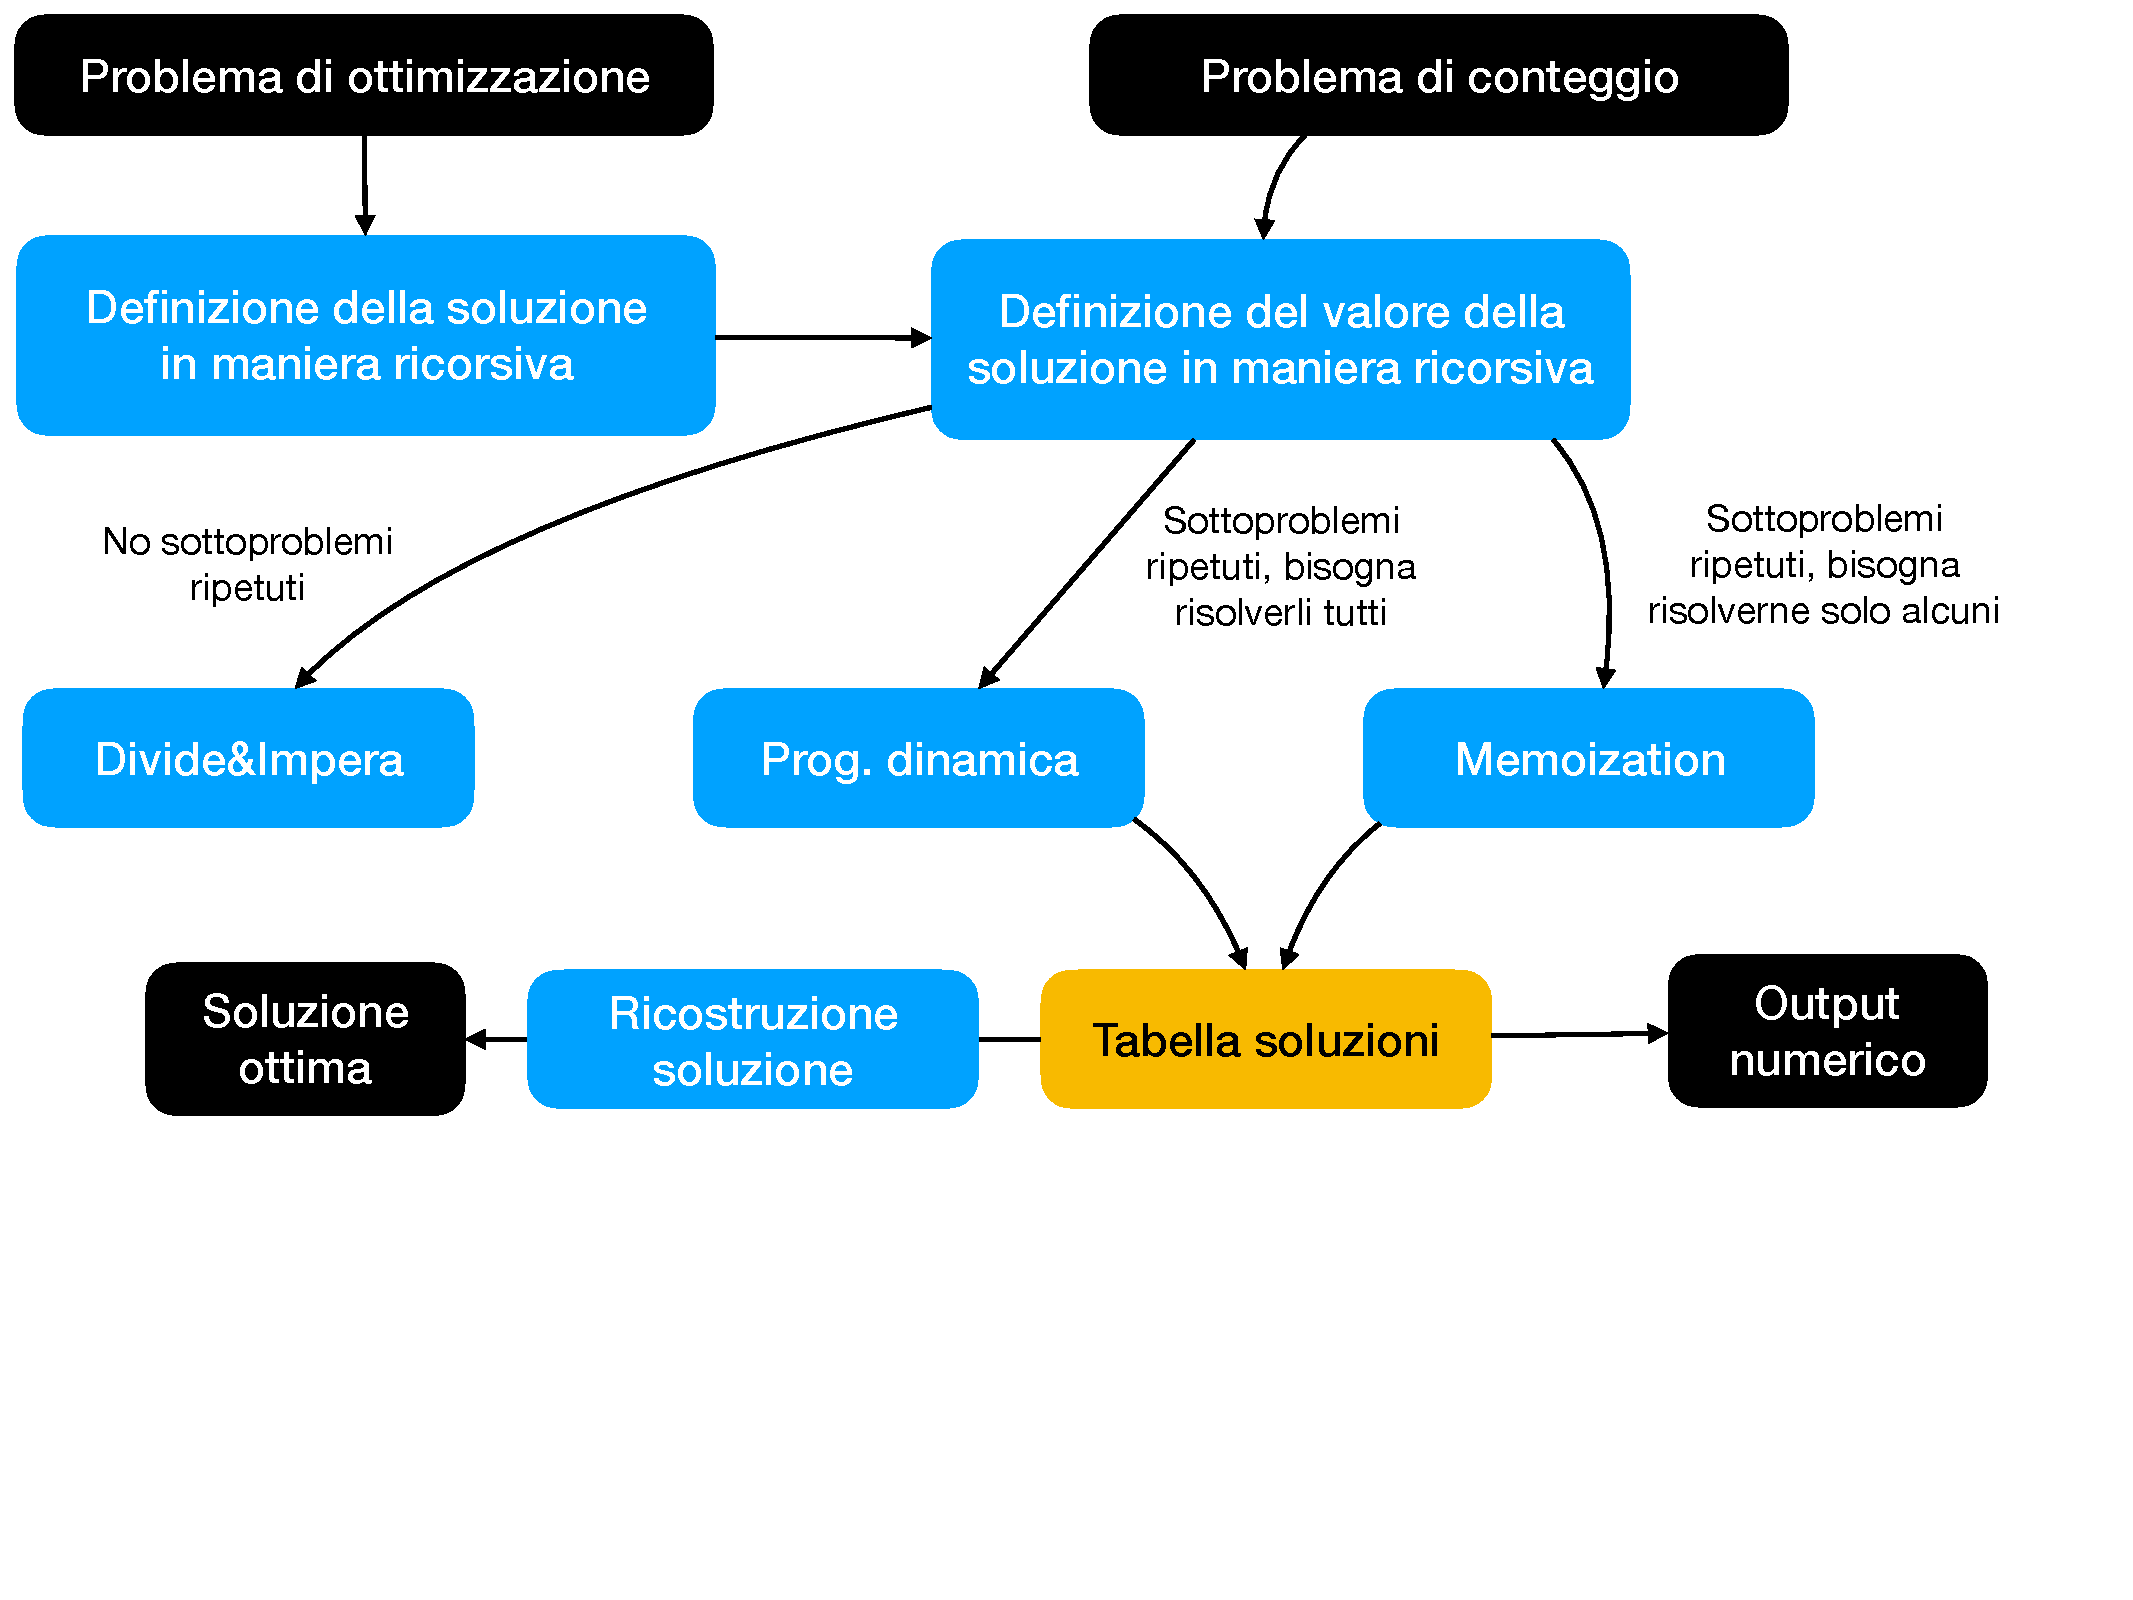
\includegraphics[width=.65\textwidth]{progrdyn}
    \end{figure}
	\item la \textbf{tecnica \foreign{greedy}} effettua sempre la scelta localmente ottima (necessita di una dimostrazione).
	\item il \textbf{backtrack} procede per \enquote{tentativi}, tornando ogni tanto sui suoi passi;
	\item nella ricerca locale la soluzione ottima viene trovata \enquote{migliorando} via via soluzioni esistenti; Negli \textbf{algoritmi probabilistici} si dimostra che talvolta è meglio scegliere casualmente, ma in modo \enquote{gratuito}, che con giudizio, ma in maniera costosa.
\end{itemize}

\section*{La tecnica del Dividi-et-Impera}

La tecnica del Divide-et-Impera si suddivide in tre fasi principali:
\begin{itemize}
	\item \textbf{Divide}: divide il problema in sotto-problemi più piccoli è indipendenti;
	\item \textbf{Impera}: risove i sottoproblemi ricorsivamente;
	\item (\textbf{Combina}): \enquote{unisce} le soluzioni dei sottoproblemi.
\end{itemize}

\ifsubfile
\end{document}
\fi